\documentclass{beamer}

% ------ Theme and Color Setup ------
\usetheme{default}
\usecolortheme{default}

% Custom colors
\definecolor{zepblue}{RGB}{0, 70, 140}
\definecolor{lightsilver}{RGB}{245, 245, 245}
\definecolor{darkgray}{RGB}{50, 50, 50}

% Gradient background
\usepackage{tikz}
\usepackage{graphicx}
\setbeamertemplate{background}{
  \begin{tikzpicture}[remember picture,overlay]
    % Light gradient
    \path[fill=white] (current page.north west) rectangle ([yshift=-0.5\paperheight]current page.north east);
    \path[fill=lightsilver] ([yshift=-0.5\paperheight]current page.north west) rectangle (current page.south east);
    % Top dark blue bar
    \fill[zepblue] (current page.north west) rectangle ([yshift=-0.7cm]current page.north east);
  \end{tikzpicture}
}

% Fonts
\usefonttheme{professionalfonts}
\usepackage{helvet}
\renewcommand{\familydefault}{\sfdefault}

% Set title and header color
\setbeamercolor{title}{fg=white}
\setbeamercolor{frametitle}{fg=zepblue,bg=white}
\setbeamercolor{item}{fg=zepblue}
\setbeamercolor{section in toc}{fg=darkgray}

% Title Page Setup
\title[Zep-CAD Project]{Zep-CAD: Mini-CAD Software for Zeppelin Modeling}
\author{Evan Blosser, Matthew Dobbs, Blake Johnson}
\institute{University of Oklahoma \\ AME 5193 - Spring 2025}
\date{\today}

\begin{document}

% ------ Title Slide ------
\begin{frame}[plain]
    \begin{tikzpicture}[remember picture,overlay]
        \fill[zepblue] (current page.south west) rectangle (current page.north east);
    \end{tikzpicture}
    \centering
    \vspace{2cm}
    {\Huge \color{white} \textbf{Zep-CAD}}\\[0.5cm]
    {\Large \color{white} Mini-CAD Software for Zeppelin Modeling}\\[2cm]
    {\large \color{white} Evan Blosser, Matthew Dobbs, Blake Johnson}\\
    {\small \color{white} University of Oklahoma \\ AME 5193 - Spring 2025}\\
    \vfill
    {\small \color{white} \today}
\end{frame}

% ------ Outline Slide ------
%\begin{frame}
    %\frametitle{Outline}
    %\tableofcontents
%\end{frame}

% ------ Sections and Slides ------

\section{Introduction}
\begin{frame}
    \frametitle{Project Objective}
    \begin{itemize}
        \item Develop lightweight Python-based CAD tool to support conceptual Zeppelin design.
        \item Enable parametric modeling and real-time surface regeneration.
        \item Provide user-friendly GUI interface using PySide6 and Matplotlib.
    \end{itemize}
\end{frame}

\section{Software Architecture}
\begin{frame}
    \frametitle{GUI Layout}
    \includegraphics[width=0.9\textwidth]{gui_layout.png}\\[0.5em]
    \small Tabbed interface with Envelope, Gondola, Engine, and Fins control panels.
\end{frame}

\begin{frame}
    \frametitle{Code Structure}
    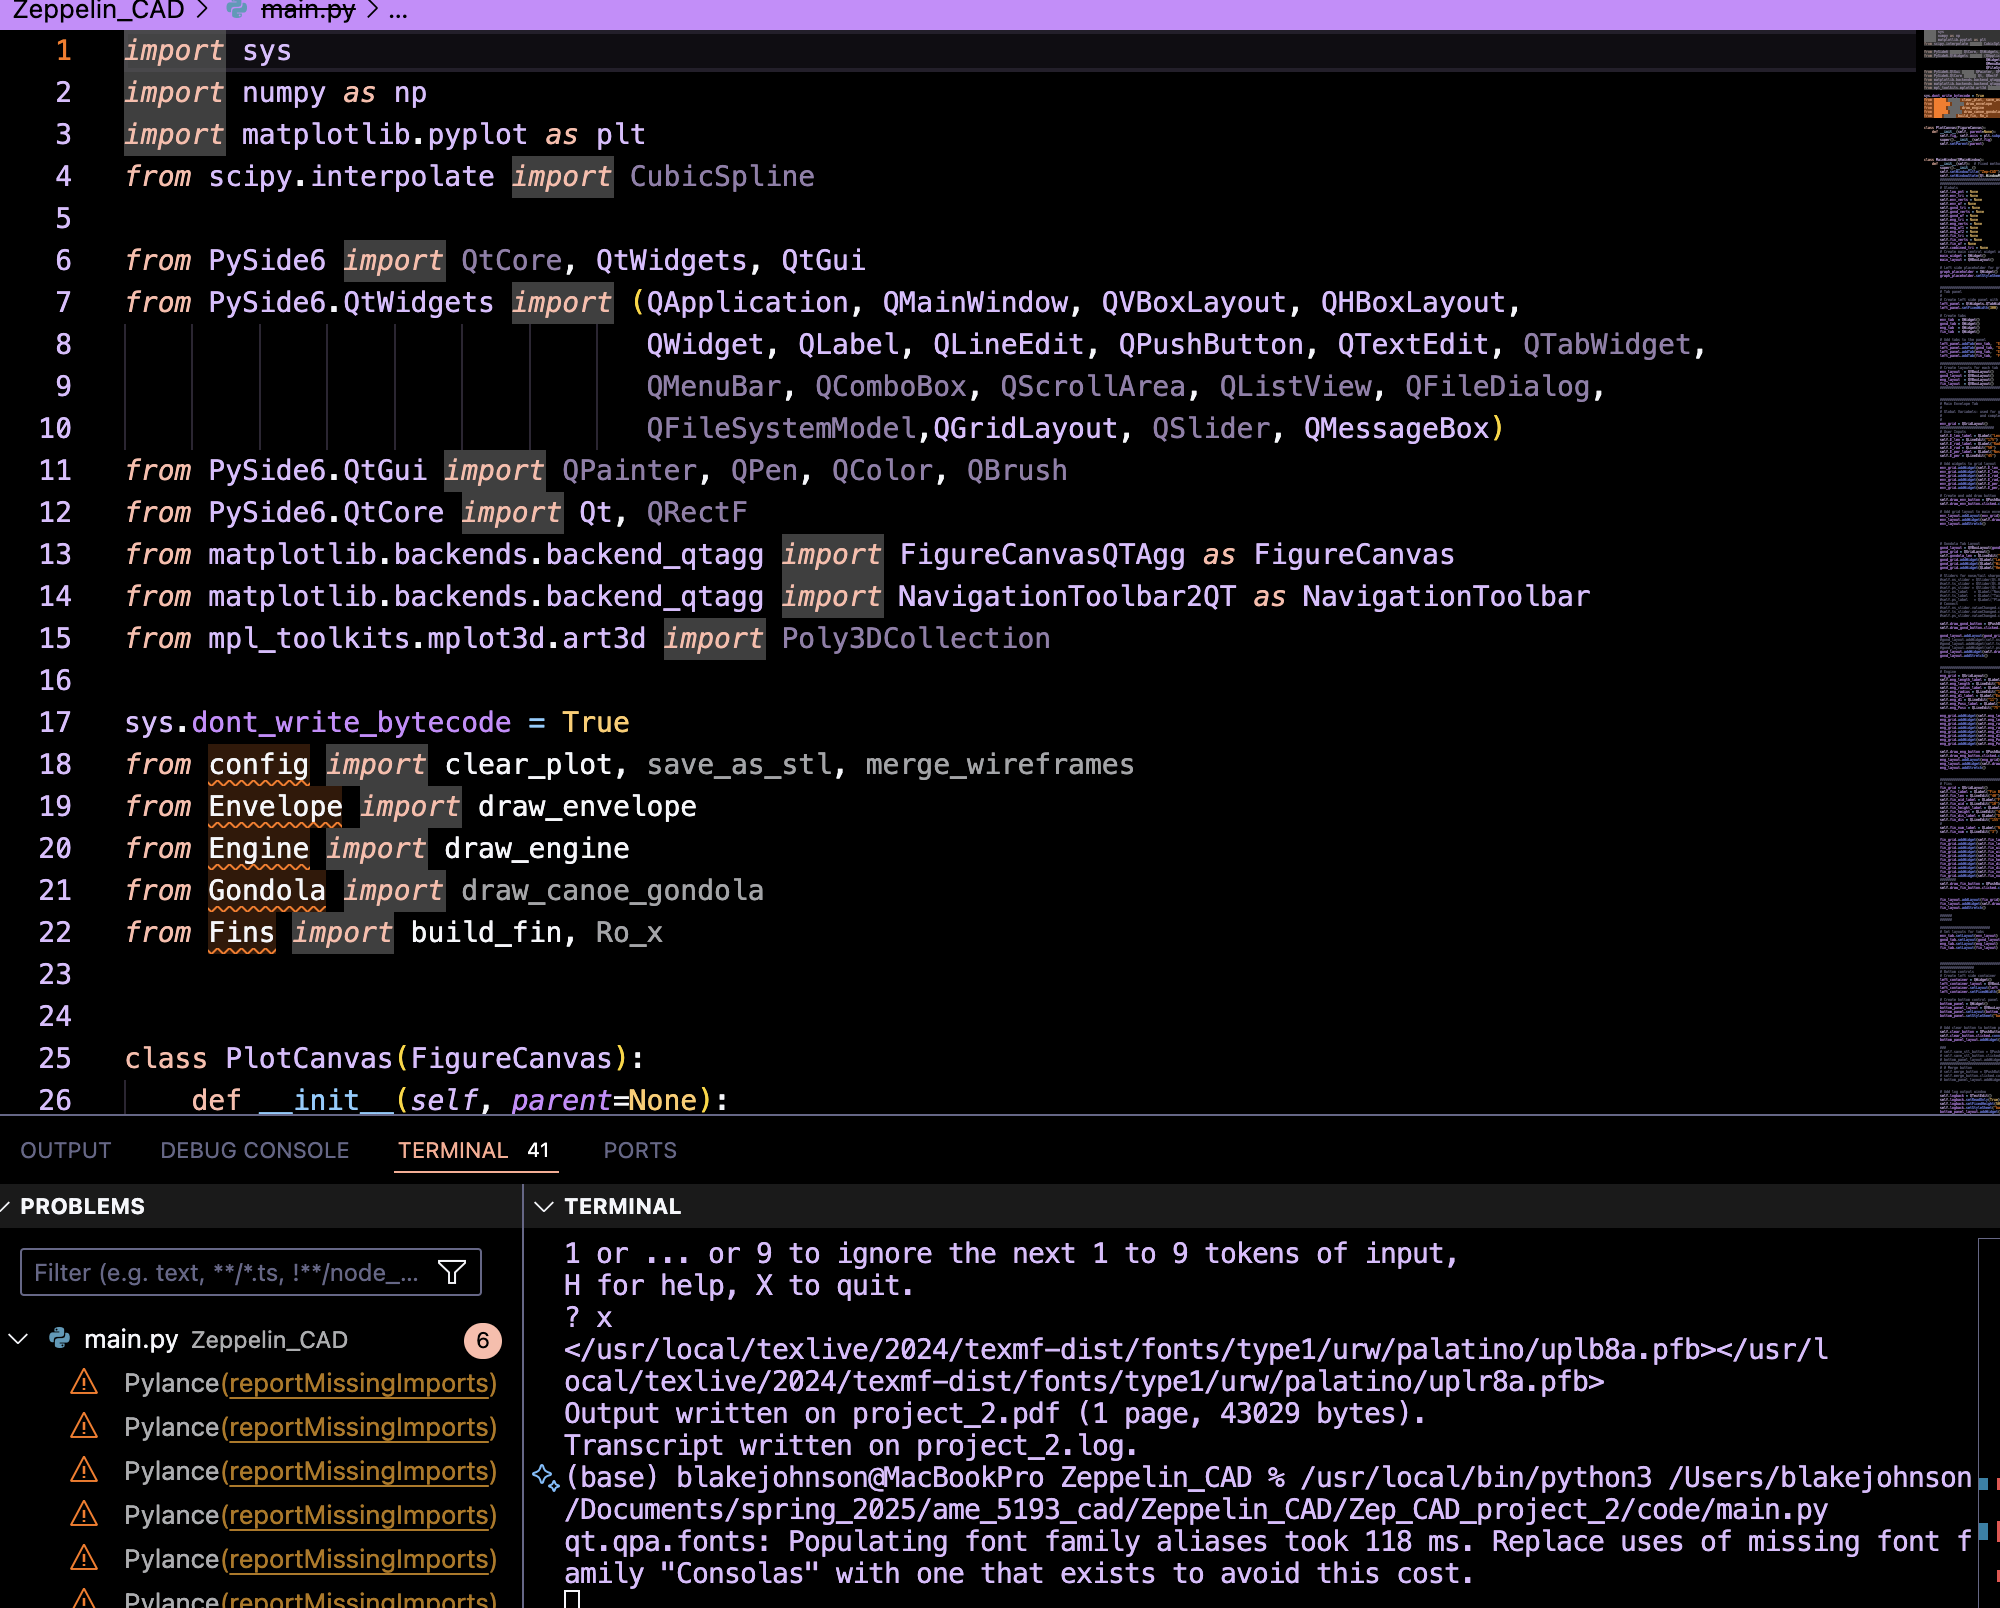
\includegraphics[width=0.9\textwidth]{code_structure.png}\\[0.5em]
    \small Modular design using main.py and independent geometry modules for each component.
\end{frame}

\section{Geometric Modeling Techniques}
\begin{frame}
    \frametitle{Curve and Surface Types}
    \begin{columns}
    \column{0.5\textwidth}
        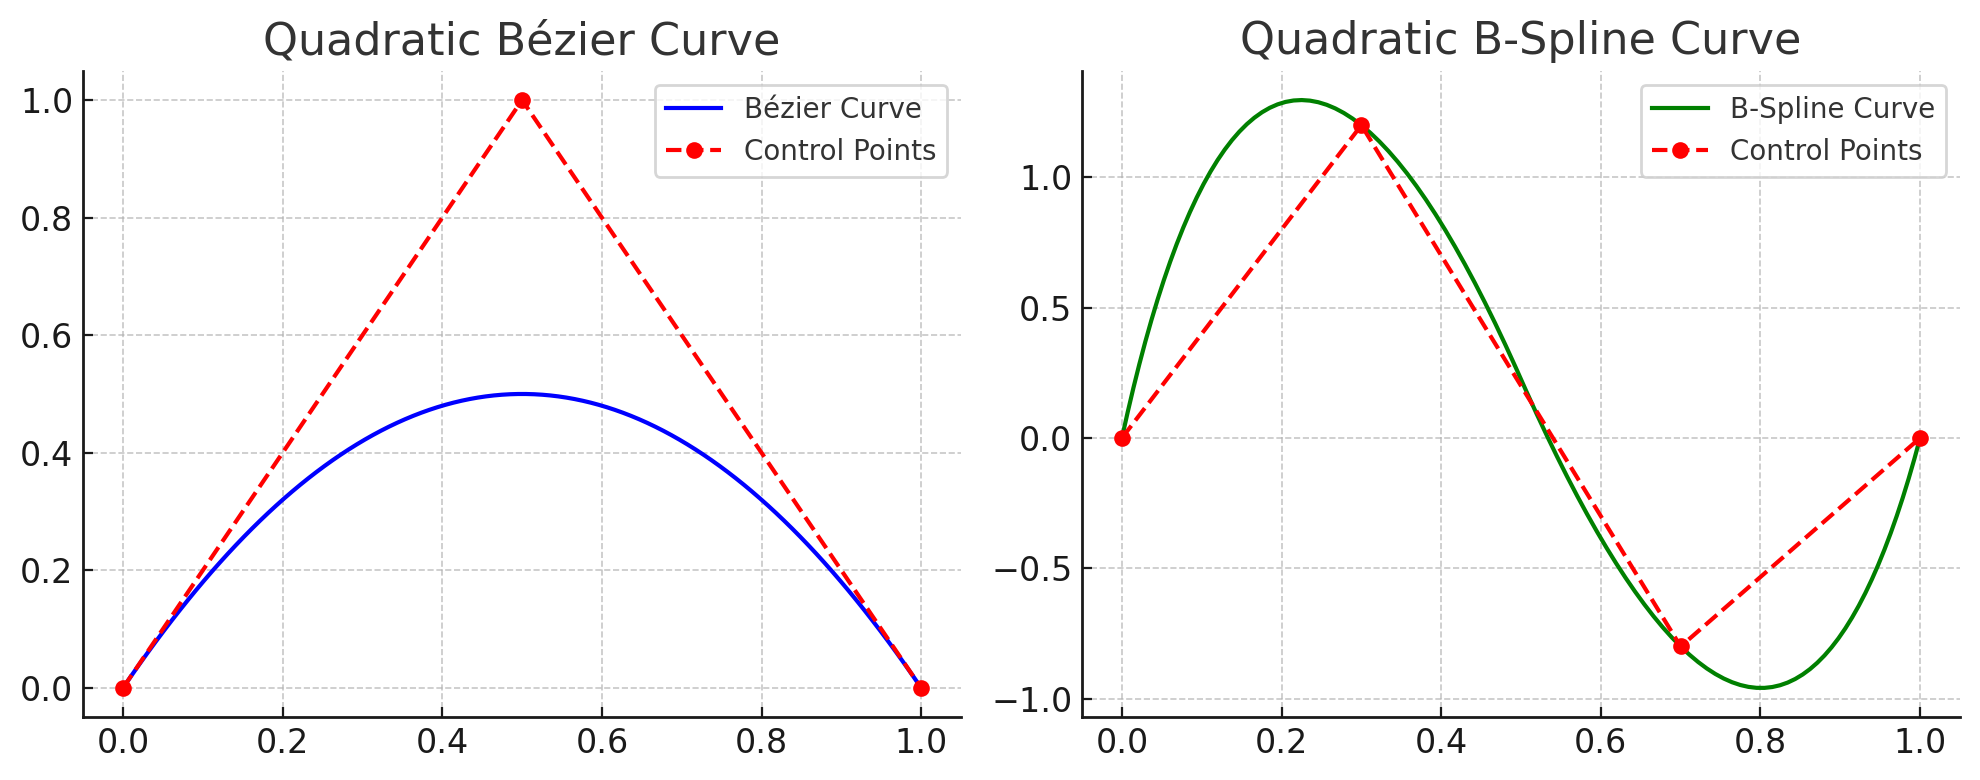
\includegraphics[width=\textwidth]{curves.png}\\
        \small\centering B\'ezier, B-spline, cubic, and quadratic spline curves.
    \column{0.5\textwidth}
        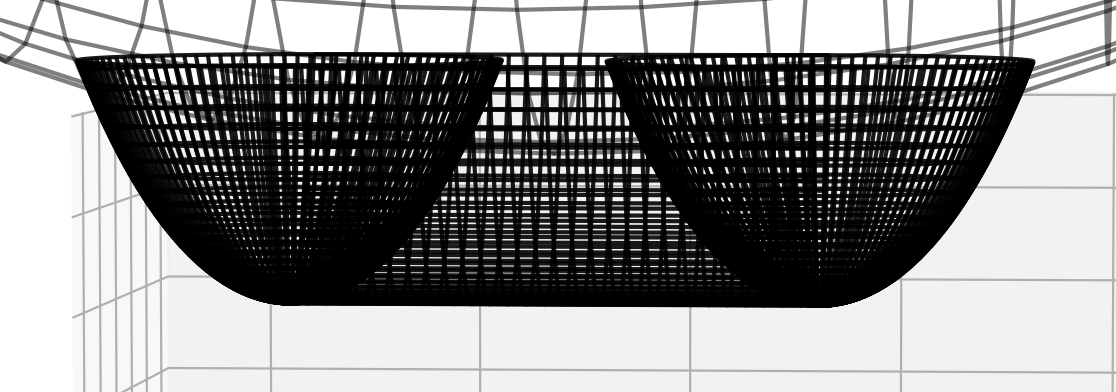
\includegraphics[width=\textwidth]{gondola_surface.png}\\
        \small\centering Revolved, ruled, and lofted surface examples.
    \end{columns}
\end{frame}

\begin{frame}
    \frametitle{Transformations}
    \begin{columns}
    \column{0.5\textwidth}
        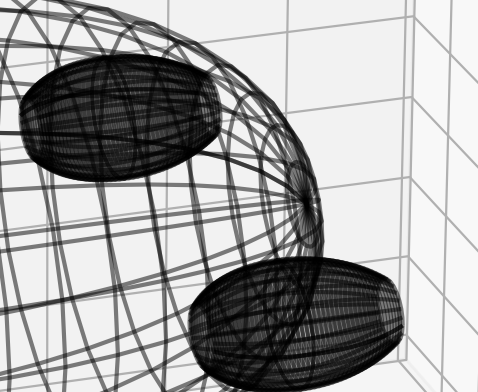
\includegraphics[width=\textwidth]{engines_close.png}\\
        \small\centering Engine translated laterally for spacing.
    \column{0.5\textwidth}
        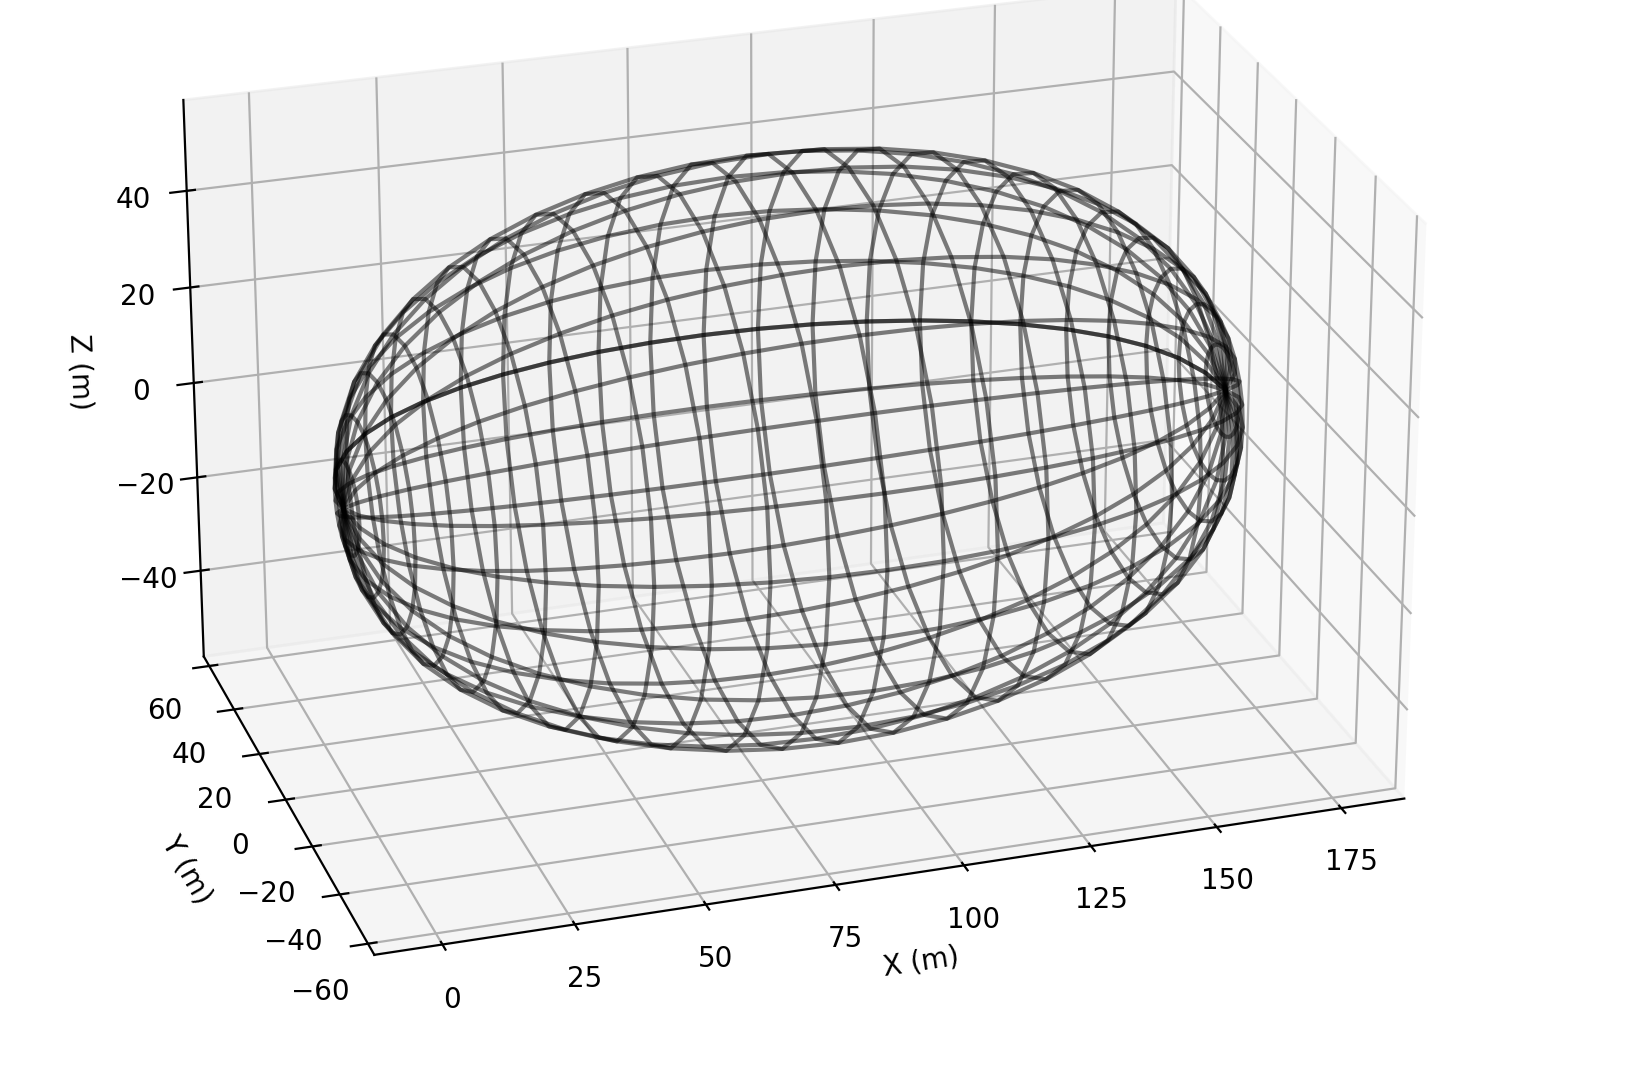
\includegraphics[width=\textwidth]{envelope_profile.png}\\
        \small\centering Fins rotated around envelope axis.
    \end{columns}
\end{frame}

\section{Proof of Concept Models}
\begin{frame}
    \frametitle{Model Variations: Nose Profiles}
    \begin{columns}
    \column{0.5\textwidth}
        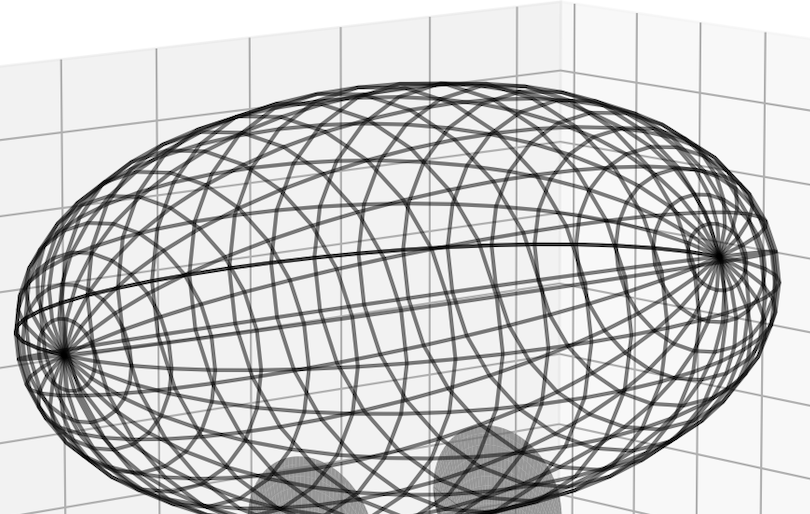
\includegraphics[width=\textwidth]{normal_nose.png}\\
        \small\centering Standard nose geometry.
    \column{0.5\textwidth}
        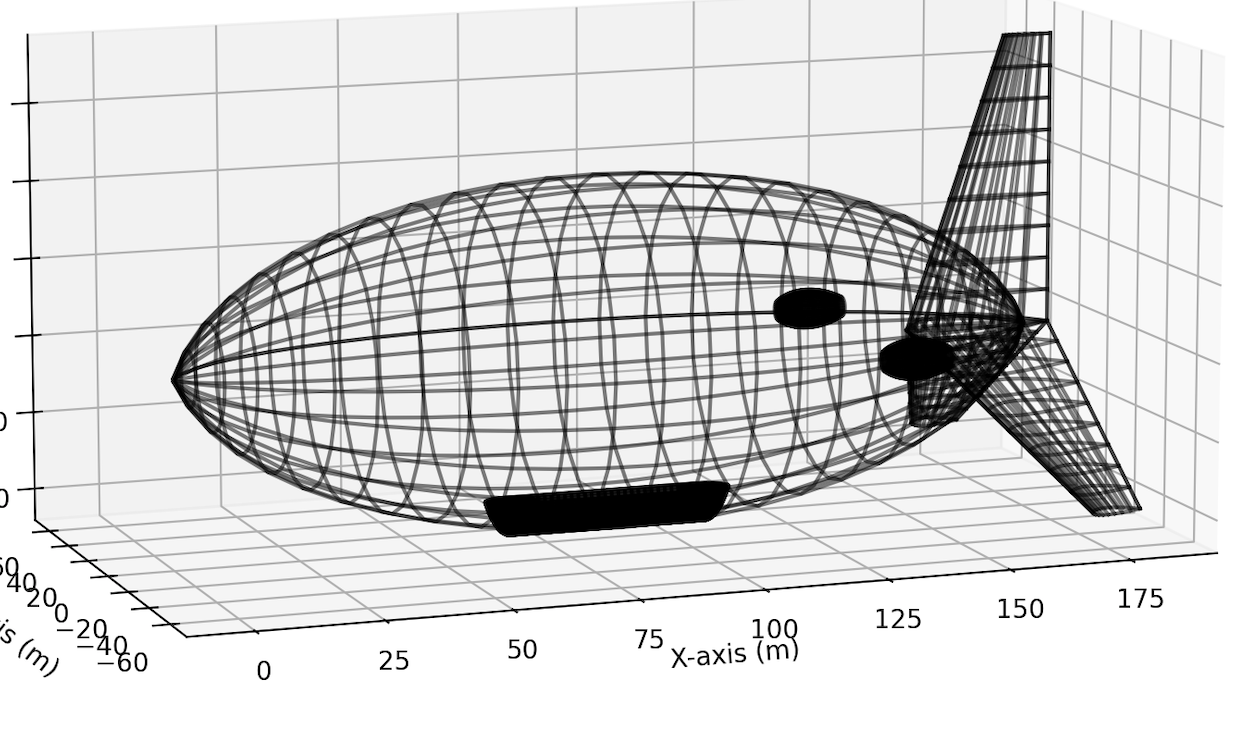
\includegraphics[width=\textwidth]{sharp_nose.png}\\
        \small\centering Sharpened nose via control point adjustment.
    \end{columns}
\end{frame}




\section{Future Work}
\begin{frame}
    \frametitle{Planned Enhancements}
    \begin{itemize}
        \item Implement gondola-envelope intersection trimming.
        \item Add STL export capabilities for 3D printing.
        \item Introduce shaded rendering and interactive rotation.
    \end{itemize}
\end{frame}

\section{Video Demonstration}
\begin{frame}
    \frametitle{Demonstration Video}
    \centering
    (Time for a Demonstration Video)
\end{frame}


\section{Conclusion}
\begin{frame}
    \frametitle{Lessons Learned}
    \begin{itemize}
        \item Integration of symbolic and numerical math for CAD.
        \item Importance of modular GUI architecture in engineering tools.
        \item Applying CAD concepts like lofting and revolving programmatically.
    \end{itemize}
\end{frame}

\begin{frame}
    \frametitle{Self-Assessment}
    \begin{itemize}
        \item Delivered a complete modular CAD prototype.
        \item Achieved real-time visual updates and user interactivity.
        \item Set groundwork for advanced features like trimming and export.
    \end{itemize}
\end{frame}

\begin{frame}[plain]
    \centering
    \Huge Thank You!\\
    \vspace{0.5cm}
    \Large Questions?
\end{frame}

\end{document}

% Continue normal slides here
